%!TEX root = ../thesis.tex
\chapter{Conclusion}
\label{chapter_conclusion}

We have presented five authoring systems for creating and following instructions from author demonstration. This final chapter restates the contributions of this dissertation and discusses the synthesis of our tools and future directions.

\section{Restatement of Contributions}
This dissertation has demonstrated video-based computational approaches that support tutorial creation and consumption. A set of interactive systems that generate concise instructions from author demonstrations are introduced. Design and technical contributions of this work can be summarized as follows:

\begin{itemize}
  \item New instructional formats that consider learning factors.
    \begin{itemize}
      \item Mixed-media tutorials composed of step-by-step static instructions and in-place video clips to demonstrate individual operations.
      \item Enhanced video playback that contains dynamic glyphs to provide viewers awareness to the upcoming input event.
    \end{itemize}
  \item Authoring workflows in an easy-to-setup environment for amateur users to create effective instructions by demonstration.
    \begin{itemize}
      \item Methods and user interfaces for recording, reviewing, and editing an instructional task with the support of software and capturing devices.
      \item Multi-modal interfaces using motion and voice commands or touch interaction to author step-by-step instructions while performing physical demonstrations.
    \end{itemize}
  \item Automatic or semi-automatic approaches using video and audio analysis that includes users in the loop to produce high-quality results.
    \begin{itemize}
      \item Algorithms of analyzing video, audio, and motion data using computer vision and signal processing approaches to segment a demonstration.
      \item Techniques for combining high-level user annotations with content analysis to generate concise instructions.
    \end{itemize}
\end{itemize}

\section{Future Directions} %Remaining Challenges and

Our tools provided evidence how computer technologies could assist amateur authors in creating instructional content, which in turns enhance the learning experiences. Based on these design experiences, we propose directions of future research in computational instruction design.

\subsection{Beyond a Single User and Linear Instructions}
The authoring systems presented in this dissertation mainly focus on supports of a single user in a software domain (i.e., MixT and DemoWiz that capture one software application walk-through) or physical tasks (including DemoDraw that records an author's movements).
%
The DemoCut system analyzes one single, static video shot. The example videos we tested included only one demonstrator. We argue that our techniques can possibly apply for content that contains multiple demonstrators' activities and narrations, but our authoring interfaces are designed for a single author.
%
Finally, the Kinectograph recording device supports two demonstrators in a scene, and the tablet interface can be possibly controlled by both users at the same time.

\subsubTitleBold{Tool Support for a Team}
We acknowledge the need of expanding our designs to support a group of authors. In specific domains, a demonstration often includes several demonstrators~\tofix{citation here}. For examples, cooking and furniture assembly tasks are commonly performed collaboratively by two or more people. Demonstrators may have different roles, such as one as the main instructor, wile the other(s) serve as supporters or a learner. For another example, dancers may have different moves in a choreography.
%
Researchers have proposed methods of detecting activities of multiple people in a video~\tofix{citation here} and video editing~\cite{PatelUIST16}, but authoring instructions collaboratively is still an open topic.
%
In addition, professional filmmaking is commonly by teamwork, where a group of people forms a production team and contributes in different stages, including planning, shooting, and editing~\tofix{citation here}. We see research opportunities in supporting large projects or complicated activities that involve long time (e.g., a few days to weeks) and multiple collaborators with the same or different roles (e.g., a director controls a recording device to document a demonstrator's making process).
% Questions here:
What information should be captured to support live or offline authoring? How should we incorporate authors' roles and intentions into a tool support? What interaction modality would be suitable to a multi-user, multi-task scenario?

\subsubTitleBold{Tool Support for Human-Robot Collaboration}
Robots have become advanced and accessible to end users for personal tasks, such as cooking~\cite{Cha:2015:RHQ:2696454.2696465} and fabricating large-scale structures~\cite{Vasey:2016:HHR:2897839.2927404}. Rather than performing a complete task individually, these robots or intelligent tools are designed to collaborate with a human user. Researchers have found that a user, who interacts with an unfamiliar robot, may confront with several challenges:
%
First, it can be difficult to understand how to operate a supportive tool or a robot during a task. Real-time guidance might be needed, especially for physical tasks. Research work has shown haptic or visual feedback to be effective for physical constructions~\cite{Agrawal:2015:PPS:2807442.2807505,Zoran:2013:FFD:2470654.2481361,Schoop:2016:DSS:2851581.2892429}.
%
Second, as tasks could involve creativity and dynamics that a human and a robot work collaboratively together, it could be challenging to foresee what a robot's next move is. Conversation~\cite{ChaoSimonSays11}, eye gaze~\cite{Andrist:2014:CGA:2559636.2559666}, and motion~\cite{Dragan:2015:ERM:2696454.2696473,Szafir:2014:CIA:2559636.2559672} enable better communications to convey robots' intent while performing a task.
%
These topics open questions to instructional design:
% Questions here:
How should instructions be presented, at what timing and in what form, when a user is working with another agent? How can a robot express it's intent while a human user is paying attention to a task?
%
We see our DemoWiz design could be one visualization method to present a robot's upcoming motion path. In fact, a recent Augmented Reality application has demonstrated this idea of visualizing a robot's trail~\cite{HoloLensRobot}, which helps users avoid collision in a space.

\subsubTitleBold{Tool Support for Alternatives}
The instructions presented in this dissertation are designed to be navigated linearly in a step-by-step order. An intriguing idea is to enable \emph{non-linear} instructions that can be interactively reviewed by a learner. Interactive narrative, or commonly known as ``Choose Your Own Adventure'', is an interactive form of dynamically following a storyline through reader's actions~\cite{RiedlInteractivenarrative}. By carefully designing a fictional world with multiple branches, readers might experience different stories, including characters, plots, and endings, based on their inputs.
%
It has been shown that such type of navigation could be useful for video editing~\cite{Shen:2009:WNE:1518701.1518825}, composing personal stories~\cite{Chi:2011:IAC:1943403.1943438}, and following educational videos~\cite{Kim:2014:DIT:2642918.2647389}.
%
As instructions involve domain knowledge and experiences, we observe that online authors have created similar forms via external links to guide viewers to other instructions. This serves several purposes, including to complete a tutorial (e.g., to pick up basic skills), to demonstrate different approaches, results, or effects, and to rise viewers' interests.
%
In addition, learners could also contribute to the instructional content via comments or edits, making a production process iterative.
% Questions here:
To support interactive navigation experiences, how would an authoring tool enable alternatives of performing a task? How would learners efficiently preview options and make a choice between approaches?
%
One useful approach is to visualize different workflows for comparison~\cite{Kong:2012:DTR:2207676.2208549} or incorporate learners' comments~\cite{Bunt:2014:TPI:2556288.2557118}, but supporting both authoring and collaborative editing for alternatives is yet an open question.

\subsection{Understanding of Expertise}
% How to design tutorial systems appropriately for different situations
% * level of expertise of instructor, learner
% * what are you trying to make easier?

\subsection{Learning from Instructions}

software learnability~\cite{Grossman:2009:SSL:1518701.1518803}
formal language
- now template, a set of techniques
machine learning

\subsection{Emerging Instructional Space}
Augmented and virtual reality systems are becoming available to end users via affordable forms. Commercial devices on the market have provided high-quality displays and inputs for VR (e.g., Oculus Rift\footnote{\url{https://www.oculus.com/}} and HTC Vive\footnote{\url{https://www.htcvive.com/}}) and AR (e.g., Microsoft HoloLens\footnote{\url{https://www.microsoft.com/microsoft-hololens/}}). 360-degree videos or spherical videos that record a complete view of a space can be captured using one omnidirectional camera or a circular array of cameras (e.g., Jump camera rig~\cite{GoogleJump}).
%
In addition, sensing technologies have been greatly improved to live track human actions~\cite{dou-siggraph2016}, hands~\cite{taylor-siggraph2016}, and locations (e.g., Project Tango~\cite{GoogleTango}) in a 3D space.
%
These enables novel applications for providing real-time instructions between people~\cite{Gurevich:2012ko,MicrosoftHoloLensSkype} and live editing and testing beyond desktop~\cite{MotionBuilderAR}.
%
However, designing AR and VR experiences extremely requires expertise and efforts in computer graphics and 3D modeling. New authoring tools that focus on delivering immersive, in-person experiences are needed.
% Questions here:
How can a tool capture a real-world demonstration and effectively transform to another remote learner? What input modality would be suitable for authoring in a physical world? How can a creation tool enable more interactive and iterative design beyond a conventional production pipeline?
%
These future directions in authoring AR and VR content are becoming more important with increasing numbers of amateur developers and authors in recent and the following years.

\begin{figure*}[ht!]
  \centering
  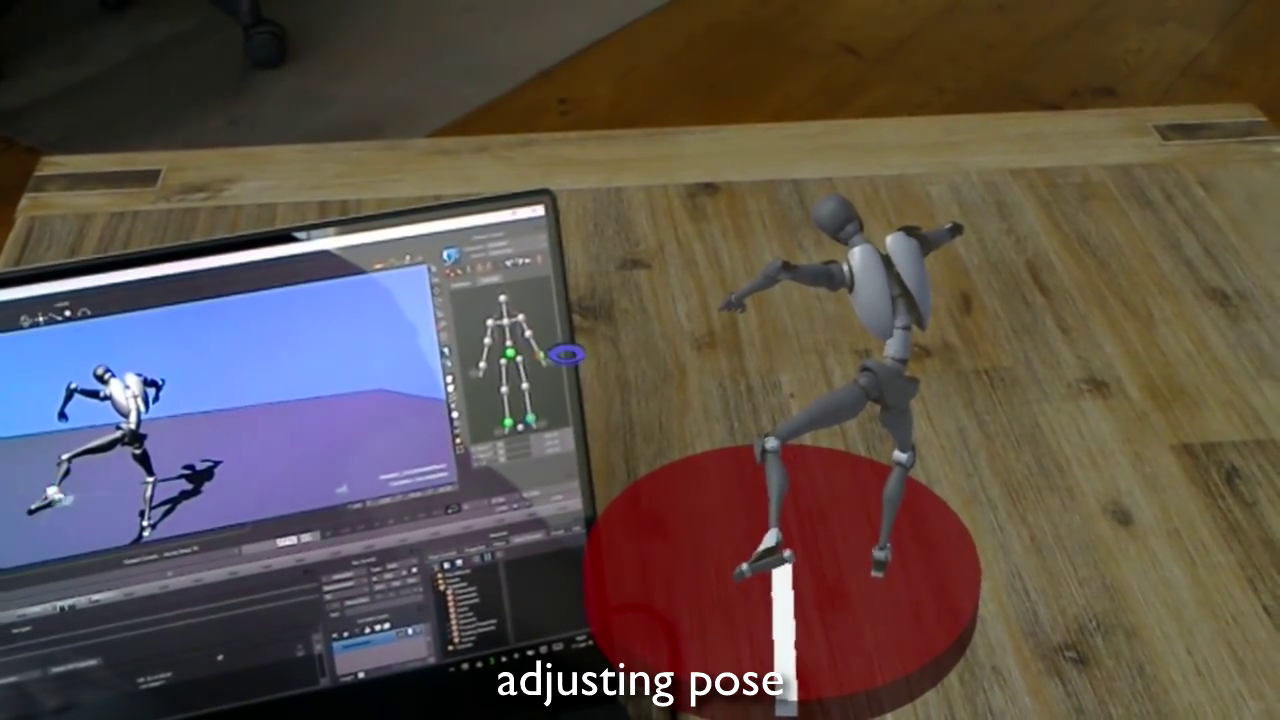
\includegraphics[width=0.45\textwidth]{\conclusion/fig/ar_authoring/motionbuilding1}
  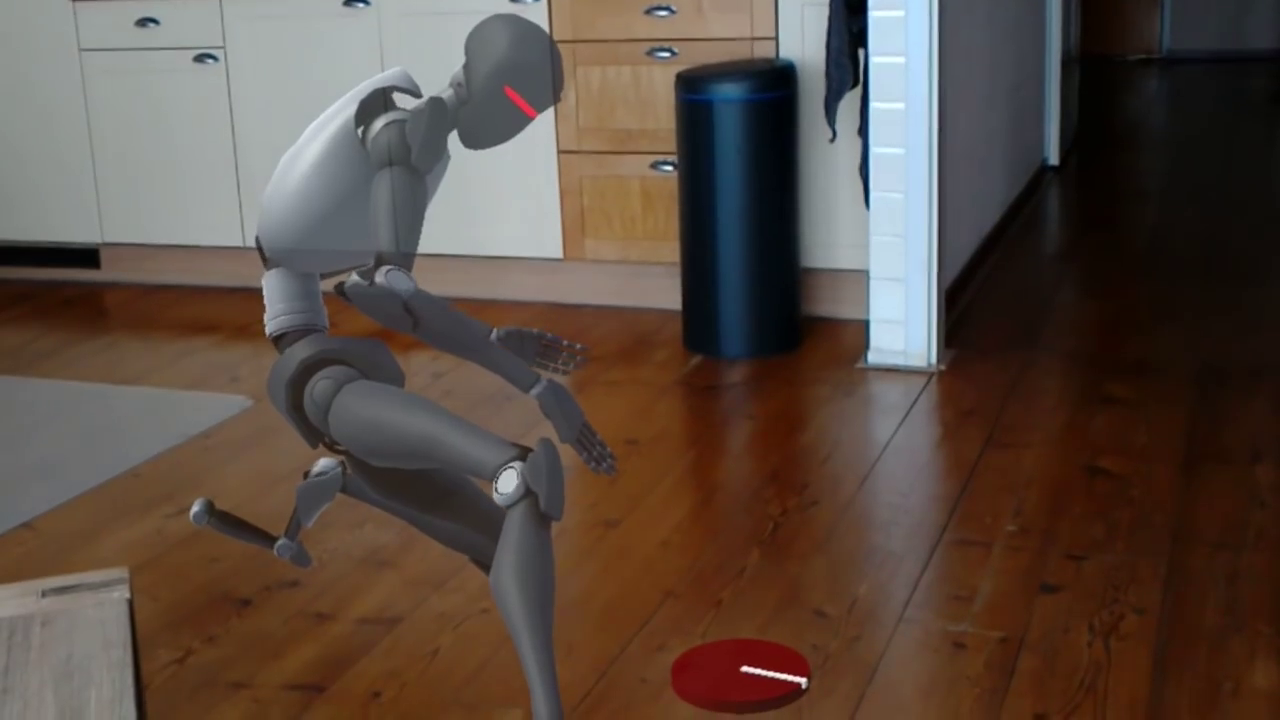
\includegraphics[width=0.45\textwidth]{\conclusion/fig/ar_authoring/motionbuilding2}
\caption{
  A recent Augmented Reality (AR) application enables reviewing character animation beyond a desktop in a room-size environment~\cite{MotionBuilderAR}, licensed under CC BY 2.0.
}
\end{figure*}

\section{Summary}
In this dissertation, we present video-based approaches designed for amateur users to produce and consume effective instructions from demonstrations. Using video and audio analysis techniques, our tools support recording, editing, and playback in a tutorial production process. We demonstrate results of a set of five computer-generated tutorials we designed for several instructional domains, including software applications and physical activities. Our results increase the quality of instructions created by tutorial authors and support learners navigating and following the tutorials.
